%%%%%%%%%%%%%%%%%%%%%%%%%%%%%%%%%%%%%%%%%%%%%%%%%%%%%%%%%%%%%%%%%%%%%%%%%%
%%%%%                         CHAPITRE 2                            %%%%%%
%%%%%%%%%%%%%%%%%%%%%%%%%%%%%%%%%%%%%%%%%%%%%%%%%%%%%%%%%%%%%%%%%%%%%%%%%%

\lhead[\fancyplain{}{\leftmark}]%Pour les pages paires \bfseries
      {\fancyplain{}{}} %Pour les pages impaires
\chead[\fancyplain{}{}]%
      {\fancyplain{}{}}
\rhead[\fancyplain{}{}]%Pour les pages paires 
      {\fancyplain{}{\rightmark}}%Pour les pages impaires \bfseries
\lfoot[\fancyplain{}{}]%
      {\fancyplain{}{}}
\cfoot[\fancyplain{}{\thepage}]%\bfseries
      {\fancyplain{}{\thepage}} %\bfseries
\rfoot[\fancyplain{}{}]%
     {\fancyplain{}{\scriptsize}}


%%%%%%%%%%%%%%%%%%%%%%%%%%%%%%%%%%%%%%%%%%%%%%%%%%%%%%%%%%%%%%%%%%%%%%%%%%
%%%%%                      Start part here                          %%%%%%
%%%%%%%%%%%%%%%%%%%%%%%%%%%%%%%%%%%%%%%%%%%%%%%%%%%%%%%%%%%%%%%%%%%%%%%%%%

\chapter{Theoretical framework}
\label{ch:2}

%==============================================================================	Résumé du chapitre

\begin{center}
\rule{0.7\linewidth}{.5pt}
\begin{minipage}{0.7\linewidth}
\smallskip

\textit{Obtaining kinematics from a network of calibrated video cameras means resolving a few theoretical points. First, features must be recognized in images. This is now mostly done with machine learning models. Then, cameras need to be calibrated, so that all of the 2D features detected for each cameras can be reconstructed in the 3D space. Finally, these coordinates must be constrained to a biomechanically consistent model, in order to obtain coherent joint kinematics.}

%\smallskip
\end{minipage}
\smallskip
\rule{0.7\linewidth}{.5pt}
\end{center}

\minitoc
\newpage


\section{Pose detection}

\subsection{Feature detection}

As a first step, achieving motion analysis from a network of cameras involves detecting features in images. These features can be whole human beings, joint centers, body landmarks, sports gear such as tennis balls, climbing holds, or much more. 

Two broad approaches can be implemented: the first one consists in using dedicated algorithms for each task. The gist of it is to understand the task well enough to build an appropriate solution. Among other techniques, corner and contour detection, color thresholding, affine transformation, template matching, watershed segmentation, can be used. For example, if one wants to differentiate two boxers wearing respectively a blue and a red shirt, they can filter them by color. If one needs to identify on which portion of a speed climbing wall an athlete is, they can match the template of each holds on the whole image. OpenCV \cite{Bradski2000} provides convenient tools for this purpose, in C++ and Python languages. This approach is often fast, but also quite complicated to implement, and neither flexible nor robust. If there is other red or blue patches in the boxing scene, if the boxer wears green or if the light is poor, this will not work anymore. Likewise for holds, if the sun casts a large shadow which changes its apparent shape, or if holds are seen from a different perspective.

The second approach takes advantage of machine learning algorithms, which constitute an entirely different paradigm. The idea is to show the machine enough examples for it to "understand" by itself its underlying attributes, so that it manages to detect and label automatically new images. This can be used for both aforementioned tasks, in a much more flexible way: if one wants the system to recognize boxers or holds in challenging condition, they simply have to include such examples while training the machine learning model. The machine learning approach is also suitable for other tasks, such as whole-image classification (i.e., determining whether this a boxing or a climbing scene), background extraction \cite{Bouwmans2019}, instance segmentation (i.e., extracting the shape of the climber, as well as each holds, the wall, the background, etc.) \cite{Minaee2021}, or keypoint detection (e.g., localization of human joint centers in an image \cite{Chen2020}). 


\subsection{Machine learning timeline and principles}

Machine learning is a subset of artificial intelligence (AI.) As such, one can trace its origin back to the discovery of the natural neuron at the end of the 19th century, by Nobel Prize Ramón y Cajal \cite{Lopez2006}, followed half a century later by the first model of an artificial neuron \cite{Mcculloch1943}. A natural neuron is a simple learning unit, which collects the nervous influx sent by other neurons to its dendrites, and sends an action potential when the total influx weighted and summed in the soma overcomes a threshold value. This potential is then transmitted through the axon to the next neuron as a new influx. Similarly, an artificial neuron receives output vectors from previous neurons, weighs and sums them with a summation function, and transfers the resulting output vector to the next neurons if it reaches a certain threshold determined by an activation function (Figure~\ref{fig_neuron}). 

The perceptron, invented in 1956 \cite{Rosenblatt1958}, represents the first practical application of an artificial neuron. It acts as a binary classifier, which automatically adjusts weights by learning from example data (see Algorithm~\ref{alg:perceptron}). It could be used, for example, to predict whether an athlete is going to be "good" or not, given his force-velocity results on an ergometer test (see step-by-step \hyperlink{example1}{Example 1} and (Figure~\ref{fig_perceptron})). 

\begin{figure}[hbtp]
	\centering
	\def\svgwidth{1\columnwidth}
	\fontsize{10pt}{10pt}\selectfont
	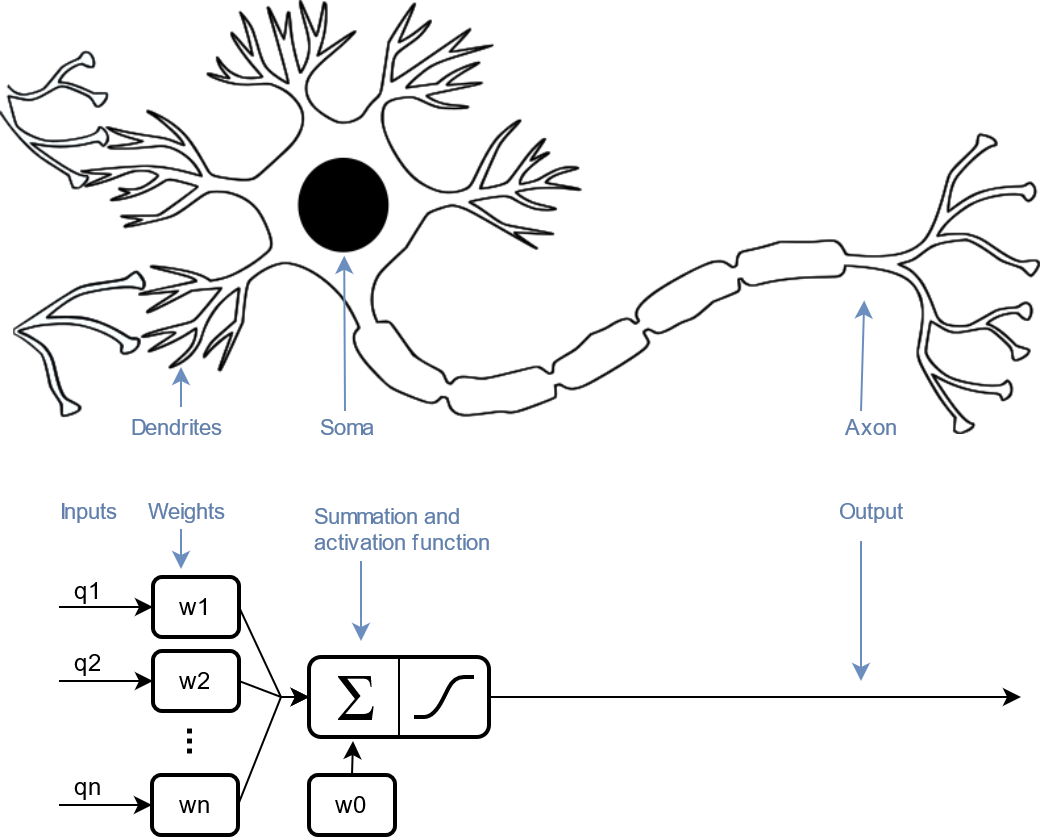
\includegraphics[width=\linewidth]{"../Chap2/Figures/Fig_neuron.png"}
	\caption{The artificial neuron has been modeled after the natural neuron. Inputs and weights act as the total nervous influx firing the dendrites. The collected values are summed, and a signal is activated if a threshold is overcome, as the soma does in a natural neuron. The output signal is conveyed through the axon.}
	\label{fig_neuron}
\end{figure}


\begin{algorithm}
      \caption{Perceptron}\label{alg:perceptron}
      \begin{algorithmic}[1]
        \STATEx Let \( \overrightarrow{X^0} \) be the input vector of a first instance of variables \( (1, x_1^0, \cdots x_m^0) \), \( \overrightarrow{W^0} \) the corresponding weights  randomly initialized \( (w_0^0, w_1^0, \cdots w_m^0) \) with \(w_0^0\) a bias, and $\sigma^{0, pred}$ the output predicted binary class. 
        \STATE The summation function is computed: 
        \begin{equation}
            \overrightarrow{W^0} \cdot \overrightarrow{X^0} = \sum_{k \in [0,m]} w_k^0 x_k^0
        \end{equation}
        \STATE This result is processed by an activation function which determines whether the neuron will be fired or not, i.e., whether one or the other class will be predicted. This is typically a threshold: 
        \begin{equation}
            \sigma^{0,pred} = 
            \begin{cases}
                1 & \text{if} \ \overrightarrow{W^0} \cdot \overrightarrow{X^0} > \theta,\\
                0 & \text{otherwise}
            \end{cases}
        \end{equation}
        \STATEx $\sigma^{0,pred}$ = 1 corresponds to one class, and $\sigma^{0,pred}$ = 0 to the other. 
        \algstore{alg1}
      \end{algorithmic}
\end{algorithm}

\begin{algorithm}
      \begin{algorithmic}[1]
        \algrestore{alg1}
        \STATE This prediction $\sigma^{0,pred}$ is compared to the actual class $\sigma^{0,actual}$. 
        \STATEx If the class is correctly predicted, then weights are retained.
        \STATEx Else, they are updated: 
        \begin{equation}
            \overrightarrow{W^1} = \overrightarrow{W^0} + \eta \ \epsilon^0 \ \overrightarrow{X^0}
        \end{equation}
        \STATEx with $\eta$ the learning rate $\in$ [0,1], and $\epsilon$ the error function. Typically, 
        \begin{equation}
            \epsilon^0 = \sigma^{0,actual} - \sigma^{0,pred}
        \end{equation}
        \STATE The algorithm is repeated with another example $\overrightarrow{X^1}$, and so on until it has gone through the whole batch of the training set. If weights still need to be updated, one can go over it again, for a determined number of epochs or until the average error is under a given value. Then the perceptron is considered trained, and ready to predict a class $\sigma$ correctly with its final weights.
      \end{algorithmic}
\end{algorithm}

\begin{tcolorbox}[colback=white,colframe=black, colbacktitle=white, coltitle=black, breakable, title=\textbf{Example 1} Perceptron, label=example1]
      \phantomsection\hypertarget{example1}
      N.B. The code for running this example is available on the thesis repository \url{http://github.com}.
      \tcblower
      Let's consider force-velocity test results as an input
      \setlength{\belowdisplayskip}{0pt} \setlength{\belowdisplayshortskip}{0pt}
      \setlength{\abovedisplayskip}{0pt} \setlength{\abovedisplayshortskip}{0pt}
      \begin{flalign*}
      \overrightarrow{X} = (1, velocity \ (m/s), force \ (hN) ), && 
      \end{flalign*}
      and the classification of an athlete as "good" or "bad" as an output
      \(\sigma = 1 \ or \ 0. \)\newline
      A  training set of n instances, i.e., example data the perceptron will learn from, could be: 
      \[ \bigl\{(\overrightarrow{X^i}, \sigma^{i, actual})\bigr\}_{i\in [0,4]}
      = \bigl\{\bigl((1, 1, 5), 1\bigr),
      \bigl((1, 2, 3), 0\bigr),
      \bigl((1, 7, 1), 1\bigr),
      \bigl((1, 4, 1), 0\bigr),
      \bigl((1, 5, 4), 1\bigr)\bigr\}. \]
      
      Let's randomly initialize weights at \(\overrightarrow{W^0} =  (-9, 1, 3) \), take a threshold $\theta$=0.1, and a learning rate $\eta$ = 0.3.\newline
        
      The first instance of the training set gives: 
      \begin{flalign*}
      \overrightarrow{W^0} \cdot \overrightarrow{X^0} = \sum\nolimits_{k \in [0,2]} w_k^0 x^0_k = -9 \times 1+ 1 \times 1 + 3 \times 5 =7.&&
      \end{flalign*}
      Now \(\overrightarrow{W^0} \cdot \overrightarrow{X^0} = 7 > \theta = 0.1\), so $\sigma^{0, pred} = 1$.\newline
      \(\sigma^{0, actual} = 1 = \sigma^{0, pred} \), so the prediction is true and weights don't need to be updated. \newline
      As a consequence, \(\overrightarrow{W^1} = \overrightarrow{W^0} = (-9, 1, 3).\)\newline
      
      The second instance gives \(\overrightarrow{W^1} \cdot \overrightarrow{X^1} = (-9, 1, 3) \cdot (1,2,3) = 2 > \theta = 0.1\), so $\sigma^{1, pred} = 1$. \newline
      But \(\sigma^{1, actual} = 0 \neq \sigma^{1, pred} = 1\), so weights need to be updated.\newline
      The error is \(\epsilon^1 = \sigma^{1,actual} - \sigma^{1,pred} = 0-1 = -1\).\newline
      As a consequence, \(\overrightarrow{W^2} = \overrightarrow{W^1} + \eta \ \epsilon^1 \ \overrightarrow{X^1} = (-9, 1, 3)  + 0.1 \times (-1) \times (1,2,3) = (-9.3,0.4,2.1).\)\newline
      
      Third instance: \(\overrightarrow{W^2} \cdot \overrightarrow{X^2} = (-9.3,0.4,2.1) \cdot (1,7,1) = 3-4.4 < 0.1\), so $\sigma^{2, pred} = 0$. \newline
      \(\sigma^{2, actual} = 1 \neq \sigma^{2, pred} = 0\), so weights need to be updated.\newline 
      \(\epsilon^2 = \sigma^{2,actual} - \sigma^{2,pred} = 1\).\newline
      \(\overrightarrow{W^3} = \overrightarrow{W^2} + \eta \ \epsilon^2 \ \overrightarrow{X^2} = (-9.3,0.4,2.1) + 0.1 \times 1 \times (1,7,1) = (-9,2.5,2.4).\)\newline
      
      Fourth instance: \(\overrightarrow{W^3} \cdot \overrightarrow{X^3} = (-9,2.5,2.4) \cdot (1,4,1) = 3.4 > 0.1\), so $\sigma^{3, pred} = 1$. \newline
      \(\sigma^{3, actual} = 0 \neq \sigma^{3, pred} = 1\), so weights need to be updated.\newline
      \(\epsilon^3 = \sigma^{3,actual} - \sigma^{3,pred} = -1\).\newline
      \(\overrightarrow{W^4} = \overrightarrow{W^3} + \eta \ \epsilon^3 \ \overrightarrow{X^3} = (-9,2.5,2.4) + 0.1 \times (-1) \times (1,4,1) = (-9.3,1.3,2.1).\)\newline
      
      \newpage

      Fifth instance: \(\overrightarrow{W^4} \cdot \overrightarrow{X^4} = (-9.3,1.3,2.1) \cdot (1, 5, 4) = 17.6 > 8\), so $\sigma^{4, pred} = 1$. \newline
      \(\sigma^{4, actual} = 1 = \sigma^{4, pred} = 1\), so weights don't need to be updated.\newline
      \(\overrightarrow{W^5} = \overrightarrow{W^4} = (-9.3,1.3,2.1) (Figure~\ref{fig_perceptron}). \)\newline

      {
      \begin{center}
      \def\svgwidth{1\columnwidth}
      \fontsize{10pt}{10pt}\selectfont
      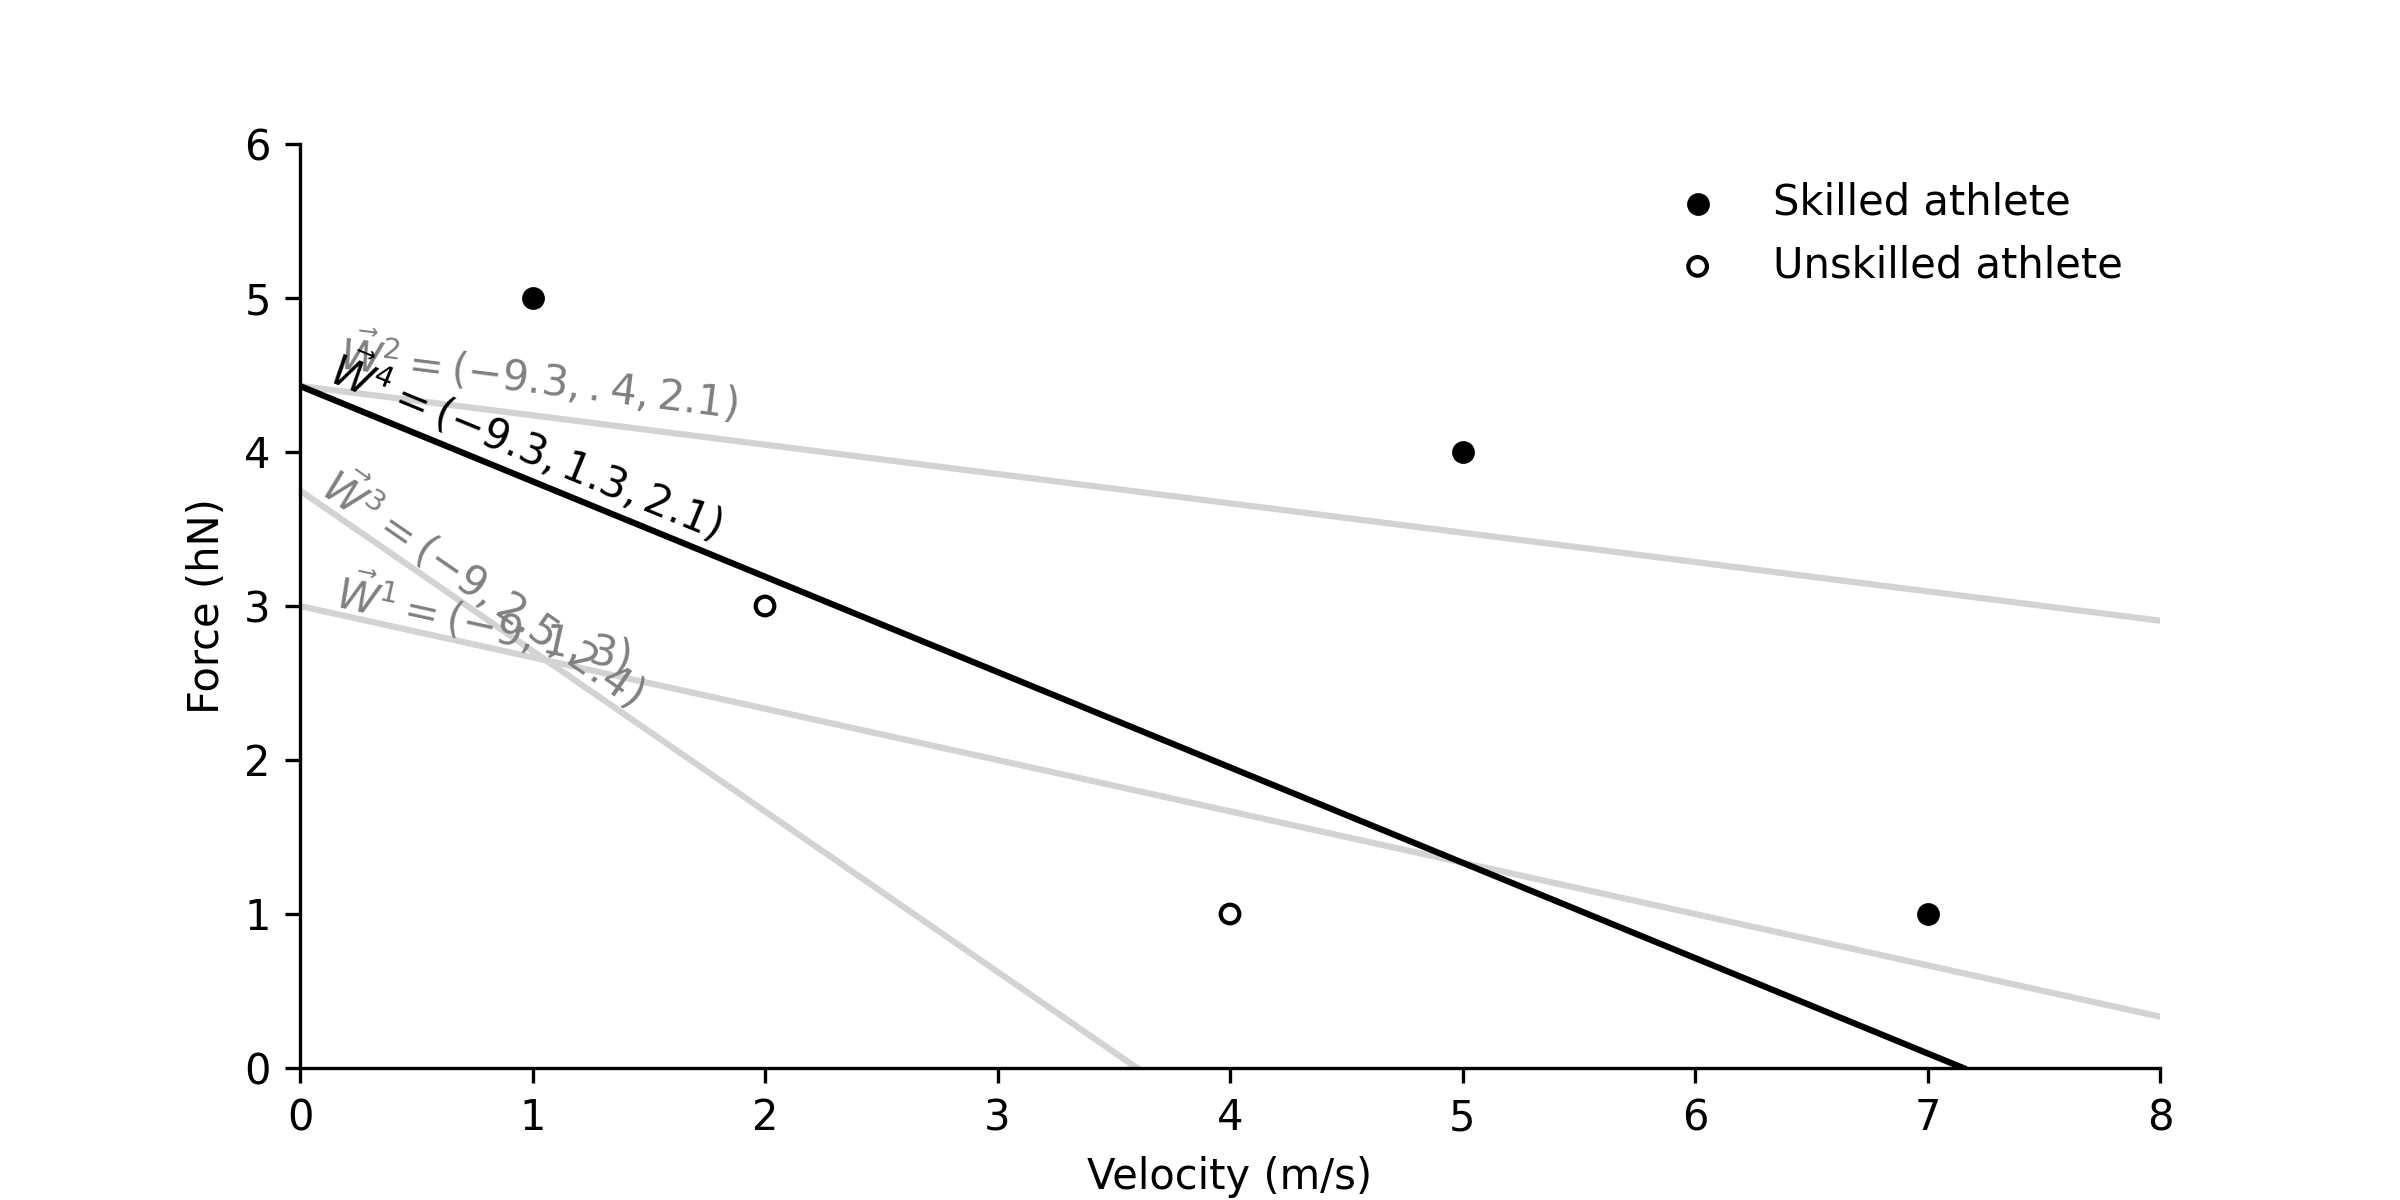
\includegraphics[width=\linewidth]{"../Chap2/Figures/Fig_perceptron.png"}
      \end{center}
      \captionof{figure}{Classification of athletes as "good" (black dot) or "bad" (circle) according to their Force-Velocity results. Weights are adjusted (grey lines), until the perceptron classifies athletes correctly (black line.)}
      \label{fig_perceptron}
      }
\end{tcolorbox}
  
% \begin{figure}[hbtp]
% 	\centering
% 	\def\svgwidth{1\columnwidth}
% 	\fontsize{10pt}{10pt}\selectfont
% 	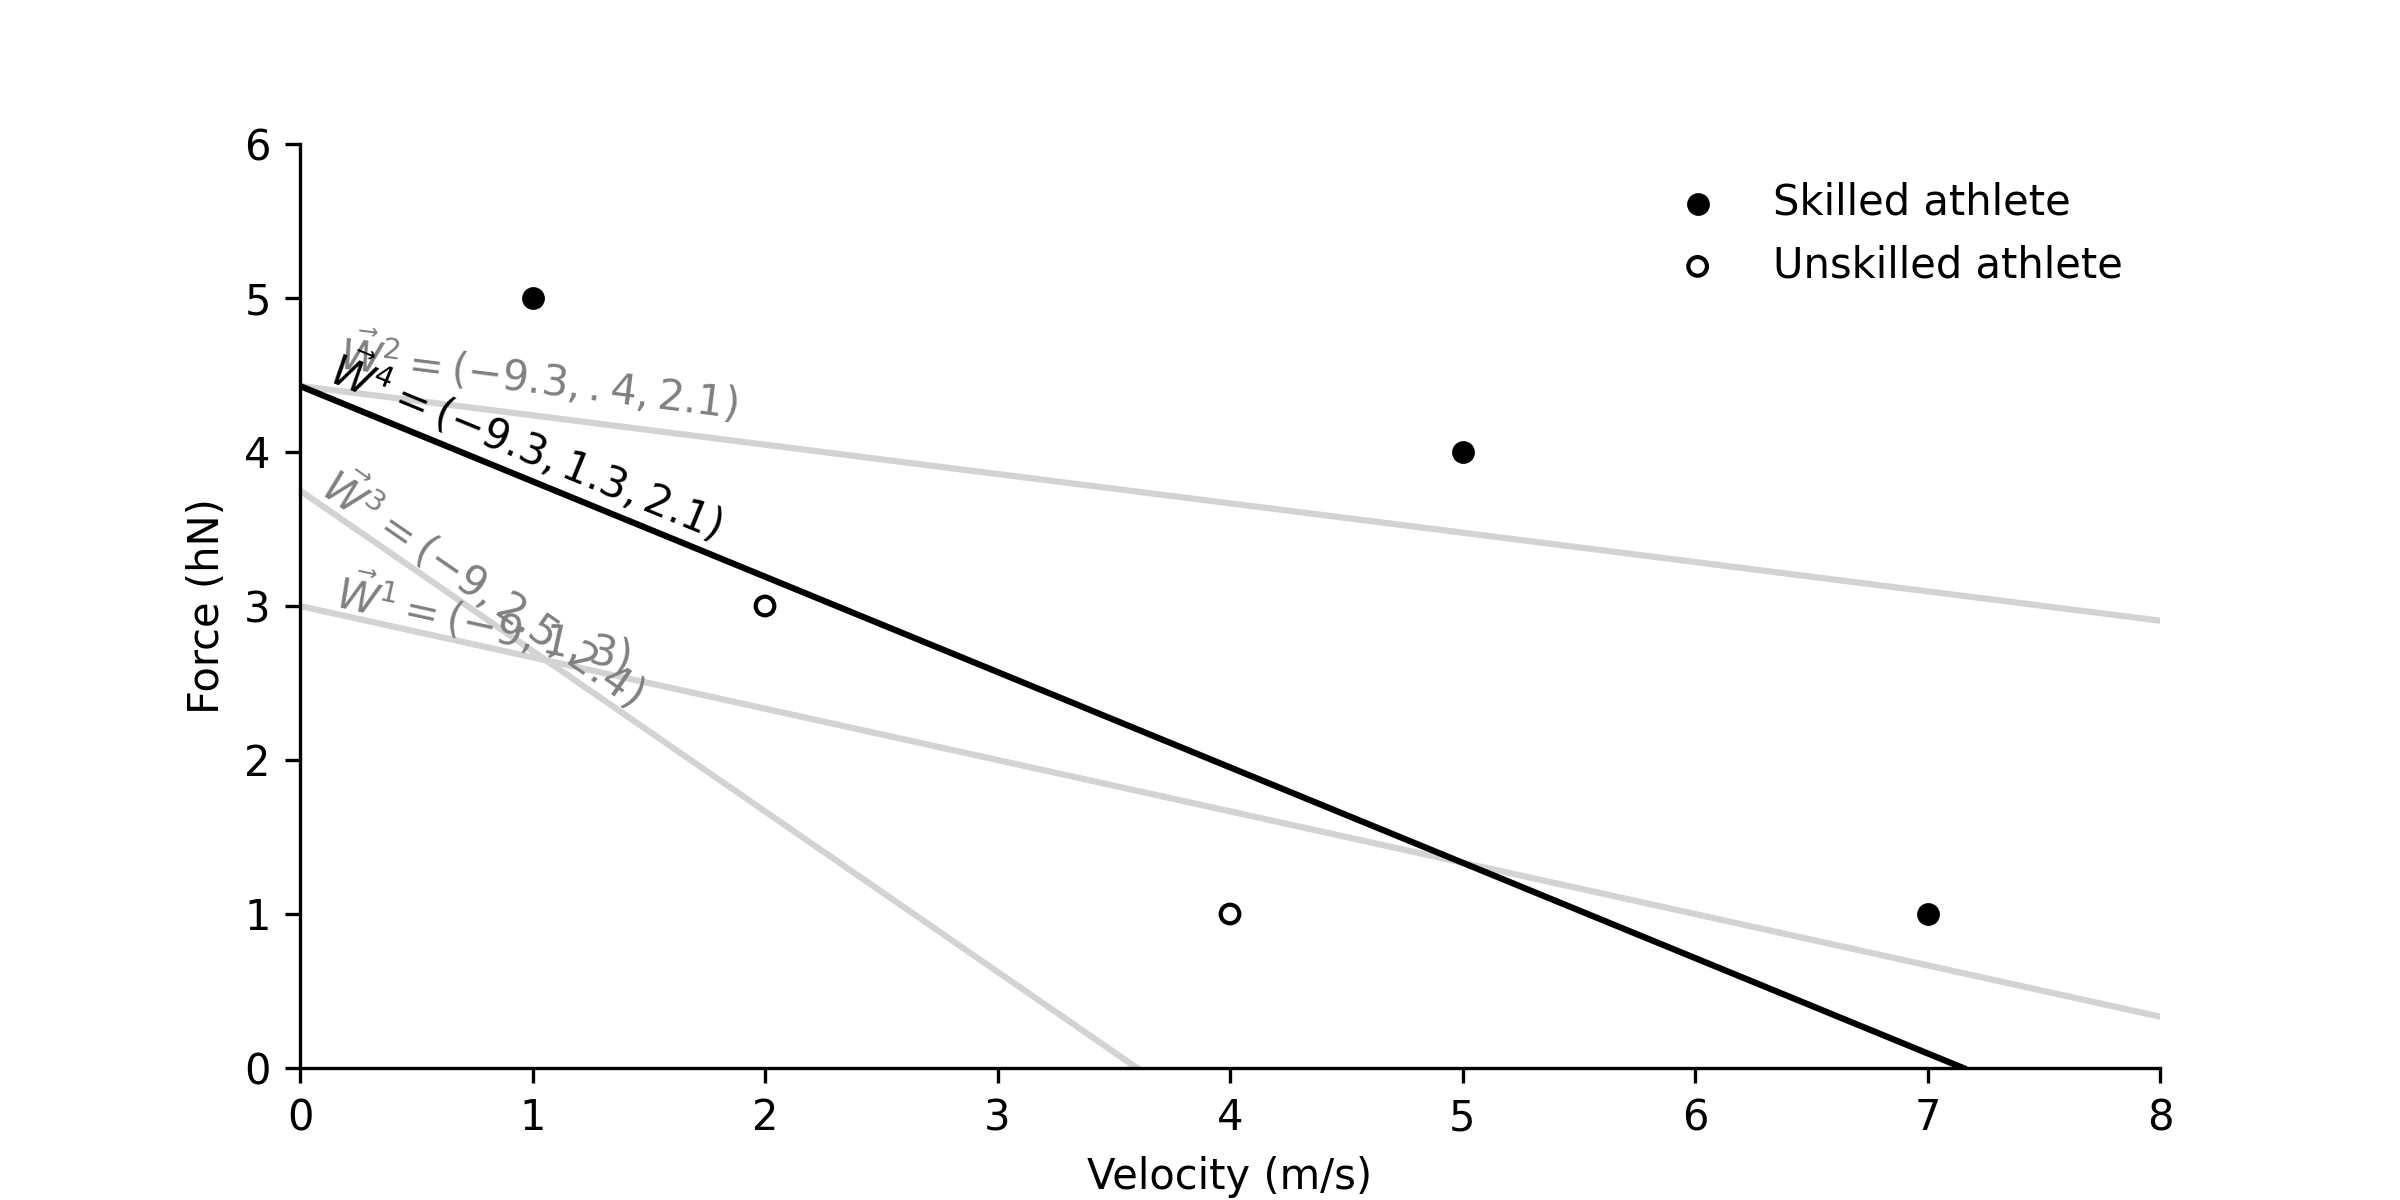
\includegraphics[width=\linewidth]{"../Chap2/Figures/Fig_perceptron.png"}
% 	\caption{Classification of athletes as "good" (black dot) or "bad" (circle) according to their Force-Velocity results. Weights are adjusted (grey lines), until the perceptron classifies athletes correctly (black line.)}
% 	\label{fig_perceptron}
% \end{figure}

% % En tikz
% \begin{figure}
% \centering
% \begin{tikzpicture}[x=0.5cm, y=0.5cm]
%     \draw[thick,->] (0,0) -- (0,6) node[anchor=south east] {Force (hN)};
%     \draw[thick,->] (0,0) -- (10,0) node[anchor=north west] {velocity (m/s)};
%     \foreach \x in {0,1,2,3,4,5,6,7,8,9}
%         \draw (\x,1pt) -- (\x,-1pt) node[anchor=north] {$\x$};
%     \foreach \y in {0,1,2,3,4,5}
%         \draw (1pt,\y) -- (-1pt,\y) node[anchor=east] {$\y$};
%     \foreach \Point in {(1,5), (5,4), (7,1)}{
%       \node at \Point {\textbullet};}
%     \foreach \Point in {(2,3), (4,1)}{
%       \node at \Point {$\circ$};}
%     % \node [green] at (5,4) {\textbullet};
%     % \node [red] at (2,3) {$\circ$};
%     \end{tikzpicture}
% \caption{Force-velocity results and classification.}
% \end{figure}

% % En matplotlib
% # Found ion https://stackoverflow.com/questions/19907140/keeps-text-rotated-in-data-coordinate-system-after-resizing
% import matplotlib.pyplot as plt
% import numpy as np
% plt.rcParams.update({'font.size': 8})
% #import matplotlib.mathtext as mathtext
% import matplotlib.text as mtext
% import matplotlib.transforms as mtransforms

% class RotationAwareAnnotation(mtext.Annotation):
%     def __init__(self, s, xy, p, pa=None, ax=None, **kwargs):
%         self.ax = ax or plt.gca()
%         self.p = p
%         self.pa = pa
%         if not pa:
%             self.pa = xy
%         self.calc_angle_data()
%         kwargs.update(rotation_mode=kwargs.get("rotation_mode", "anchor"))
%         mtext.Annotation.__init__(self, s, xy, **kwargs)
%         self.set_transform(mtransforms.IdentityTransform())
%         if 'clip_on' in kwargs:
%             self.set_clip_path(self.ax.patch)
%         self.ax._add_text(self)

%     def calc_angle_data(self):
%         ang = np.arctan2(self.p[1]-self.pa[1], self.p[0]-self.pa[0])
%         self.angle_data = np.rad2deg(ang)

%     def _get_rotation(self):
%         return self.ax.transData.transform_angles(np.array((self.angle_data,)), 
%                             np.array([self.pa[0], self.pa[1]]).reshape((1, 2)))[0]

%     def _set_rotation(self, rotation):
%         pass

%     _rotation = property(_get_rotation, _set_rotation)

% plt.figure(figsize=(8, 4))
% plt.axis([0, 8, 0, 6])
% plt.gca().spines['top'].set_visible(False)
% plt.gca().spines['right'].set_visible(False)
% plt.gca().set_xlabel('Velocity (m/s)')
% plt.gca().set_ylabel('Force (hN)')

% velocity_good = [1,5,7]
% force_good = [5,4,1]
% velocity_bad = [2,4]
% force_bad = [3,1]
% plt.scatter(velocity_good, force_good, s=20, edgecolors='k', facecolors='k', label = "Good athlete")
% plt.scatter(velocity_bad, force_bad, s=20, edgecolors='k', facecolors='none', label="Bad athlete")
% plt.legend(frameon=False)

% # First lines with first weights, with dash greyed lines and label
% W=[-9,  1,  3]
% x1 = np.array( [0, -W[0]/W[1]] )
% x2 = np.array( [-W[0]/W[2], 0] )
% plt.plot(x1,x2, 'lightgrey')
% RotationAwareAnnotation(r'$\vec{W}^1=(-9,1,3)$', 
%       xy=(.15,3.3), p=[-W[0]/W[1],0], pa=[0,-W[0]/W[2]], ax=plt.gca(), xytext=(2,-1), textcoords="offset points", va="top", c='grey', bbox=dict(facecolor='None', edgecolor='None'))
    
% W=[-9.3, .4,  2.1]
% x1 = np.array( [0, -W[0]/W[1]] )
% x2 = np.array( [-W[0]/W[2], 0] )
% plt.plot(x1,x2, 'lightgrey')
% RotationAwareAnnotation(r'$\vec{W}^2=(-9.3, .4,  2.1)$', 
%       xy=(.15,4.85), p=[-W[0]/W[1],0], pa=[0,-W[0]/W[2]], ax=plt.gca(), xytext=(2,-1), textcoords="offset points", va="top", c='grey', bbox=dict(facecolor='None', edgecolor='None'))

% W=[-9,  2.5, 2.4]
% x1 = np.array( [0, -W[0]/W[1]] )
% x2 = np.array( [-W[0]/W[2], 0] )
% plt.plot(x1,x2, 'lightgrey')
% RotationAwareAnnotation(r'$\vec{W}^3=(-9,2.5,2.4)$', 
%     xy=(.15,4), p=[-W[0]/W[1],0], pa=[0,-W[0]/W[2]], ax=plt.gca(), xytext=(2,-1), textcoords="offset points", va="top", c='grey', bbox=dict(facecolor='None', edgecolor='None'))

% W=[-9.3,  1.3, 2.1]
% x1 = np.array( [0, -W[0]/W[1]] )
% x2 = np.array( [-W[0]/W[2], 0] )
% plt.plot(x1,x2, 'k')
% RotationAwareAnnotation(r'$\vec{W}^4=(-9.3,  1.3, 2.1)$', 
%       xy=(.15,4.75), p=[-W[0]/W[1],0], pa=[0,-W[0]/W[2]], ax=plt.gca(), xytext=(2,-1), textcoords="offset points", va="top", bbox=dict(facecolor='None', edgecolor='None'))

% plt.savefig(r'D:\softs\github_david\latex\These\fichiers_latex\Chap2\Figures\Fig_perceptron', dpi=300)
% plt.show()




\newpage

Of course, the example below is oversimplified. Being good or not as a sport is multifactorial, and the model would be more exact if more variables were taken into account. 

Learning rate, threshold
training data size (and quality), number of epochs to run on a batch (i.e., a subset of the training data)
activation function, error (gradient descent)
only linearly separable
multilayer

% This is the basis of the supervised learning paradigm, which is the most common one in machine learning. The perceptron is a linear classifier, which means that it can only separate two classes of data with a straight line. This is why it is often used as a first step in a more complex classification problem, such as the one of recognizing a human pose in an image.

% This is the idea behind the multilayer perceptron (MLP), which was invented in 1969 \cite{Rumelhart1986}. This is a neural network composed of several layers of neurons, which can be used to classify data in a more complex way. For example, if one wants to classify athletes according to their performance in a 100m sprint, they could use the time, the force-velocity results, the body mass, the height, the age, etc. as input variables. The first layer of neurons would be used to classify the athletes according to their force-velocity results, the second layer would classify them according to their time, and so on. The output layer would then be used to classify them according to their performance.







It would need as a prior some example data

Given a training set, it could learn
It could be used, for example, to classify whether an athlete is powerful or not, given his test results on 

The perceptron rule is 


Let's consider an input \(\overrightarrow{X} = \begin{pmatrix} 1 \\ 5 \end{pmatrix} \)

\begin{equation} 
      h = w_0 + \overrightarrow{w} \cdot \overrightarrow{q} 
\end{equation}
      
\begin{equation} 
      \overrightarrow{w^{t_1}} = \overrightarrow{w^{t_0}} + r\, c\, \overrightarrow{q^{t_0}} 
\end{equation}
      
\begin{multline}
      \biggl\{(\overrightarrow{q_i}, \overrightarrow{c_i})\biggr\}_{i\in [1,n]} \\
      = \Biggl\{ 
      \biggl( \begin{pmatrix} 1 \\ 5 \end{pmatrix}, 1 \biggr),
      \biggl( \begin{pmatrix} 2 \\ 3 \end{pmatrix}, -1 \biggr),
      \biggl( \begin{pmatrix} 4 \\ 1 \end{pmatrix}, -1 \biggr),
      \biggl( \begin{pmatrix} 5 \\ 4 \end{pmatrix}, 1 \biggr),
      \biggl( \begin{pmatrix} 8 \\ 1 \end{pmatrix}, 1 \biggr)
      \Biggr\}
\end{multline}
      
      
in hN and in m/s
      
\begin{equation}
      h(\overrightarrow{q}) = 
      \begin{cases}
      1 & \text{if} \ w_0 + \overrightarrow{w} \cdot \overrightarrow{q} > 0,\\
      0 & \text{otherwise}
      \end{cases}
\end{equation}


w0 biais

Limitation


Possible de jouer sur le learning rate (adaptive?), sur les poids initiaux, ainsi que sur la fonction d'activation (exemple: sigmoïde) et sur la fonction d'erreur, biais, multilayer?

Pas possible si non linéairement séparable (exemple image)

Define learning step $\eta$ 

Winters 1966 and 1988 (XOR, Turing, power, funding)
"the spirit is willing but the flesh is weak." Translated back and forth with Russian, it became "the vodka is good but the meat is rotten." during cold war. Dictionary without context

CNN

Deep learning

-> perceptron mono/multicoucheNeurone: unité d'apprentissage



History natural neuron and formal neuron (dates, names, comparison)

Timeline cahier jaune et wiki

S'inspirer de wikipedia (en, fr, timeline); 
S'inspirer du mail machine learning starred (exemple du réseau de neurones); 
S'inspirer du cahier jaune


- deep learning vs CNN (vs SVM, random forest, etc.), AI, machine learning

- classification vs detection vs segmentation

data augmentation, dropout, batch normalization
overfitting
train / test
accuracy loss
gradient descent
layers, batch size, epochs, activation

transfer learning

% \subsection{Application to object detection and localization}


\subsection{Pose detection}

Different architectures, different models, different datasets


\section{3D reconstruction}\label{sec:3D reconstruction}

While some approaches only rely on 2D pose estimation to infer 3D pose with another machine learning model, they are generally not considered to be sufficiently reliable. It is, then, important to use the input from several cameras, and to fuse their informations to obtain 3D coordinates.


\subsection{Pinhole camera model}

Voilà


\subsection{Calibration}

test


\subsection{Triangulation}

suite


\section{3D joint kinematics}

\subsection{Physically consistent model}

autre


\subsection{Scaling}

bref


\subsection{Inverse kinematics}

As opposed to forward kinematics \newline
Compare with 2D angles between 3 points \newline
Different methods (model based vs autres) for angles (cf mail starred)\newline




